\documentclass[a4paper,14pt ]{article} % можно использовать кегель 8-12, 14, 17 и 20 пунктов
\DeclareMathSizes{14}{14}{14}{14}
\usepackage{extsizes}
\usepackage{graphicx}
\graphicspath{{/home/misha/VUZ/TOE/laby/l3/osc/}}
\usepackage[russian]{babel} % задаёт русский как основной язык текста
\usepackage[T2A]{fontenc} % задаёт кириллическую кодировку шрифта
\usepackage{cmap} % обеспечивает нормальное копирование и поиск русского текста в pdf 
\usepackage[utf8]{inputenc} % определяет юникодную кодировку самого .tex-файла
\setcounter{secnumdepth}{0}
\usepackage{geometry} % задаёт поля 
\geometry{left=3cm} % левое — 3 см
\geometry{right= 1.5cm} % правое — 1,5 см
\geometry{top=2cm} % верхнее — 2 см
\geometry{bottom=2cm} % нижнее — 2 см
\usepackage{setspace} \onehalfspacing % задаёт «полуторный» межстрочный интервал 
\usepackage{indentfirst} % автоматически добавляет отступ в каждый новый абзац
\usepackage{amsmath,amsfonts,amssymb,amsthm,mathtools,mathtext, physics}
\usepackage{float}
\usepackage{array}
\usepackage{tabularx}
\usepackage{titlesec}
\titleformat{\section}{\centering\normalfont\bfseries}{\thesection}{1em}{}
\titleformat{\subsection}{\centering\normalfont\bfseries}{\thesection}{1em}{}
\titleformat{\subsubsection}{\centering\normalfont\bfseries}{\thesection}{1em}{}
\setlength\parindent{1.25cm}
\begin{document} 
\begin{titlepage}
    \begin{center}
        {\bf  МИНОБРНАУКИ РОССИИ\\
        САНКТ-ПЕТЕРБУРГСКИЙ ГОСУДАРСТВЕННЫЙ\\
        ЭЛЕКТРОТЕХНИЧЕСКИЙ УНИВЕРСТИТЕТ\\
        <<ЛЭТИ>> ИМ. В. И. УЛЬЯНОВА (ЛЕНИНА)\\
    
        }
    \end{center}
    \vfill
        {
        \begin{center}
            \bfseries
            ЛАБОРАТОРНАЯ РАБОТА №3\\
            по дисциплине <<Теоретические основы электротехники>>\\
            Тема: <<ИССЛЕДОВАНИЕ СВОБОДНЫХ ПРОЦЕССОВ
            В ЭЛЕКТРИЧЕСКИХ ЦЕПЯХ>>\\
        \end{center}
        }
        \
    \vfill
        {\noindent\parbox{4cm}{Студенты гр. 3114}  \hfill \parbox{3cm}{\rule{3cm}{0.15mm}} \hfill \parbox{4cm}{\raggedleft Злобин М. А.\\ Федулова Л. В. \\ Раузер А. А.}} \\\\
        \parbox{4cm}{Преподаватель} \hfill \parbox{3cm}{\rule{3cm}{0.15mm}} \hfill \parbox{4cm}{\raggedleft Лановенко Е. В.} \\ 
        \center Санкт-Петербург
        
        2025
\end{titlepage}
Цель работы: изучение связи между видом свободного процесса
в электрической цепи и расположением ее собственных частот 
(корней характеристического уравнения) на комплексной плоскости; 
экспериментальное определение собственных частот и добротности RLC-контура 
по осциллограммам. 


В работе предлагается исследовать свободные процессы в цепях, схемы
которых представлены на рис. \ref{fig:1} Цепи возбуждаются короткими импульсами тока
$i_0(t)$, заряжающими конденсатор C. В паузах между импульсами
конденсатор разряжается; цепь находится в свободном режиме, так как в это
время источник возбуждения отключен
$i_0 = 0$
. Напряжения на элементах
цепи осциллографируются.
Поведение линейных цепей описывается линейными дифференциальными уравнениями;
 при этом вид свободного процесса определяется корнями $p_k$
характеристического уравнения (собственными частотами цепи).
\begin{figure}[H]
    \centering
    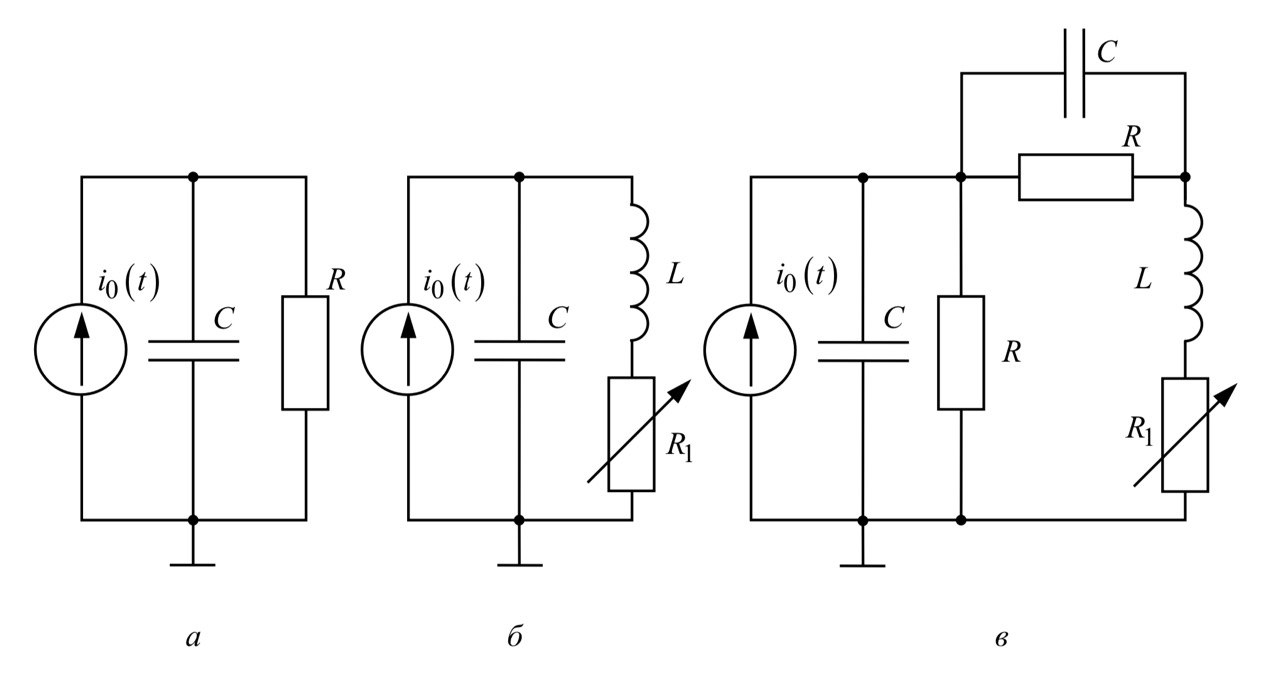
\includegraphics[width=1\linewidth]{cheme}
    \caption{Схемы, исследуемые в работе}
    \label{fig:1}
\end{figure}
\section{Исследование свободных процессов в цепи первого порядка (рис. \ref{fig:1}, a)}
\subsection{Расчет собственной частоты цепи по осциллограмме}
\begin{figure}[H]
    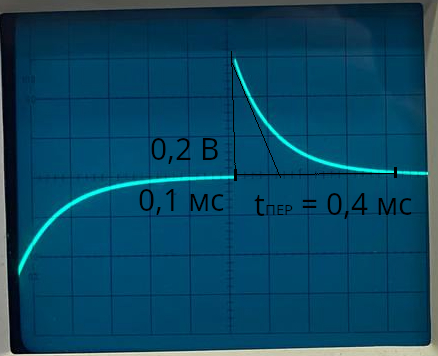
\includegraphics[width=0.6\textwidth]{11p}
    \centering
    \caption{\centering Осциллограмма реакции системы. Черными метками отмечена длительность
    переходного процесса}
\end{figure} Т. к. $t_\text{пер} = 3\tau = 0.4 \text{ мс}$, $\tau = 0.133\text{ мс}
\implies p_1 = -\dfrac{1}{\tau} = -7500\text{ Гц}$
\subsection{Теоретический расчет собственных частот}
\begin{table}[h]
    \centering
    \begin{tabular}{|r|c|c|l|}
        \hline
        $R = 5 \text{ кОм}$ & $C = 0.02 \text{ мкФ} $ & $ U = 8 \text{ B}$ &
        $\dfrac{1}{f} = T = 1.2 \text{ мс} $ \\
        \hline
    \end{tabular}
    \caption{параметры цепи 1-го порядка и входного импульса}
\end{table}
Собственные частоты можно найти как нули входной проводимости $Y(p)$:
$ Y(p) = pC + \frac1R $, откуда $ p_1 = -\alpha = -1/(RC) $.

$p_1 = -1/(5\cdot10^3\cdot0.02\cdot10^{-6}) =  -10^{4}$ Гц.
\begin{enumerate}
    \item Аналитический процесс описывается выражением $f_2(t) = Ae^{-7500t}$.
    \item Порядок теоретической и экспериментальной часот совпал.
\end{enumerate} \newpage
\section{Исследования свободных прцессов в цепи 2-го порядка (рис. \ref{fig:1}, б)}
К элементам, которые перечислены в таблице 1 добавляем {\it L} -- элемент со значения 25 мГн.
\subsection{Расчет собственных частот в колебательном режиме} 
\begin{figure}[H]
    \centering
    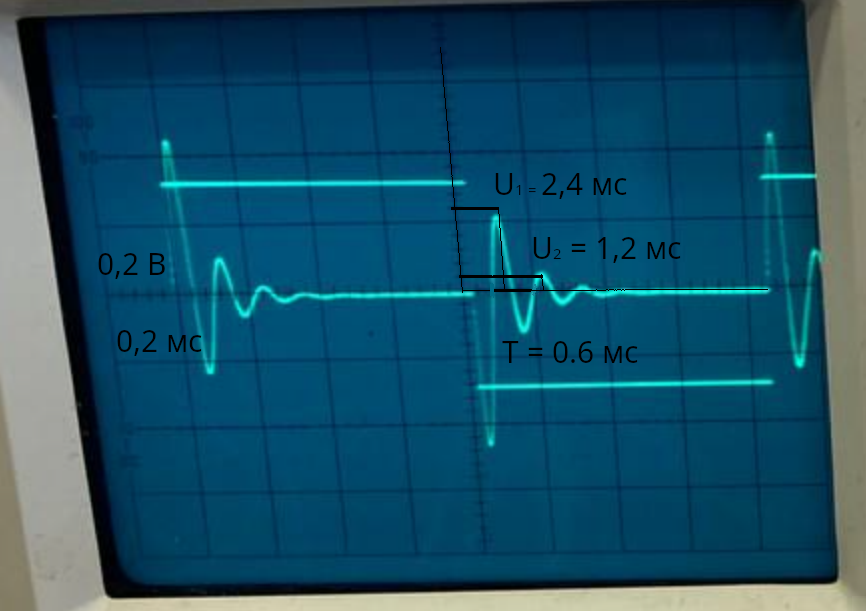
\includegraphics[width=1\textwidth]{2pp.png}
    \caption{\centering Осциллограмма колебательного затухающего процесса в цепи второго порядка}
\end{figure}
Найдем $\alpha = \ln\left(\dfrac{U_1}{U_2}\right)\cdot\dfrac1T = \ln\dfrac{0.02}{0.22}
1/(0.12\cdot10^{-3}) = -19982.4 \,\, c^{-1}
$.
\\\\
\indentНайдем $w = \dfrac{2\pi}{T} = \dfrac{2\pi}{0.12\cdot10^{-3}} = 52360$ Гц.
\\\\
\indent Таким образом, $p_{1,2} = 10^3\cdot(-20 \pm i52)$.
\\\\ 
\indent Теоретический расчет: 
\begin{multline*}
    \alpha = -\dfrac{R_1}{2L} 
= -\dfrac{0.5\cdot10^3}{25\cdot10^{-3}} = -20000;\\ 
w_0 =\dfrac1{\sqrt{LC}} = 
= \dfrac{1}{\sqrt{25\cdot10^{-3}\cdot0.02\cdot10^{-6}}} =  44721; \\w = 
\sqrt{\alpha^2 - w_0^2} = 39999.5. 
\end{multline*}
\indent Добротность контура при {\it R} = 0.5 кОм:
\begin{equation*}
    Q=\frac{2\pi}{2\alpha T} = \frac{2\pi}{2\cdot39965\cdot 0.06 \cdot 10^{-3}}=
    1.31
\end{equation*}
\indent Теоретическая добротность контура: 
\begin{equation*}
    Q = \frac{\sqrt{L/C}}{R} = \dfrac{\sqrt{25\cdot10^{-3}/0.02/10^{-6}}}{0.5\cdot10^3} = 2.2.
\end{equation*}
\indent Добротность контура при {\it R} = 0 (колебательный незатухающий режим):
\begin{equation*}
    Q = \frac{2\pi}{2\alpha T} \to \infty
\end{equation*}
\subsection{Расчет собственных частот в апериодическом режиме}
$p_{1,2} = -\alpha \pm \sqrt{\alpha^2 - w_o^2} = -60000 \pm 40000$. 
\subsection{Расчет собственных частот в критическом режиме}
\begin{figure}[H]
    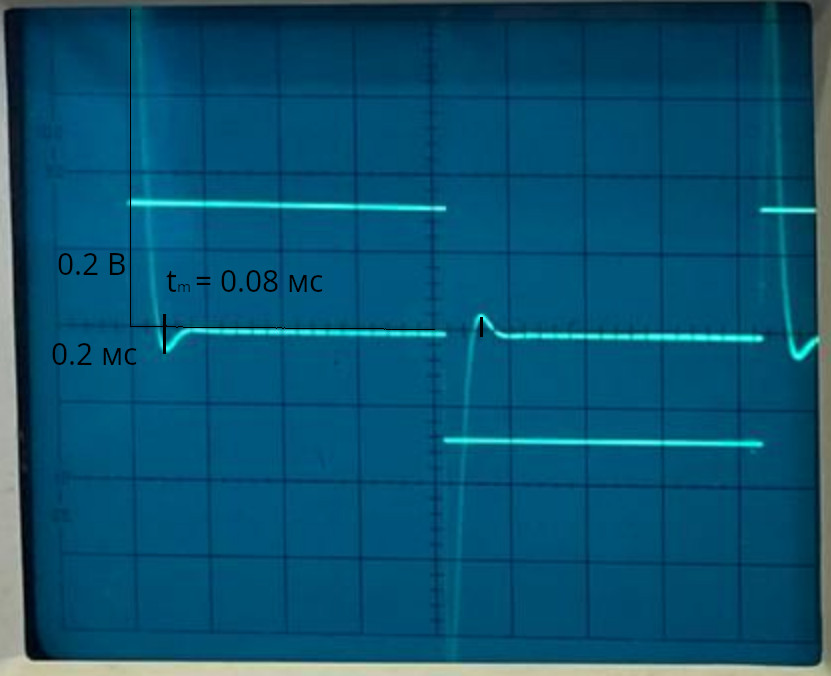
\includegraphics[width=1\textwidth]{3pp}
    \centering
    \caption{Осицллограмма процесса при критическом режиме в цепи 2-го порядка}
\end{figure}
Расчитаем $\alpha = -\dfrac1{t_m} = -\dfrac1{0.04\cdot10^{-3}}= -12500 \implies p_{1,2} = -12500$. 
\\\\ \indent Tеоретическое значение собственные частот в критическом режиме:
\begin{equation*}
    \alpha = -\frac{R_1}{2L} = -\frac{1.5\cdot10^3}{2\cdot25\cdot10^{-3}} = -30000.
\end{equation*}
\begin{enumerate}
    \item В периодическом режиме: $f_2(t) = A_1e^{(-20 + i52)\cdot 10^3t} + A_2e^{(-20 + i52)\cdot 10^3t}$;
    \\В апериодическом режиме: $f_2(t) = A_1e^{-20000t} + A_2e^{-100000t}$;
    \\В критическом режиме: $f_2(t) = Ae^{-12500t} + A_1e^{-12500t}t$.
    \item $p_{1,2} = 20000, 100000$, этим значения соотвествует осциллограмма.
    \item Оба значения близки и соотвествуют условию $Q > 0.5$, характерного для колебательного режима.
 \end{enumerate}    
\section{Расчет собственных частот в цепи 3-го порядка}
\section{Колебательный режим} 
\begin{figure}[H]
    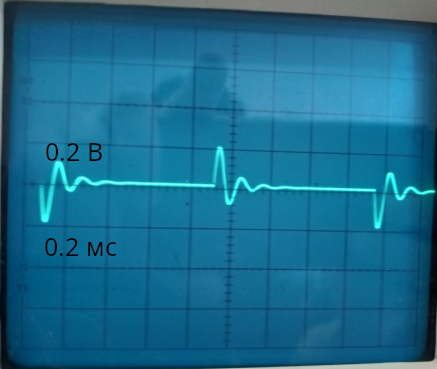
\includegraphics[width=0.7\linewidth]{4pp}
    \centering
    \caption{Периодический режим в цепи 3-го порядка}
\end{figure}
Расчитаем собственные частоты для периодического режима цепи 3-го порядка:
\begin{multline*}
    p_1 = -\frac{1}{RC} = \frac{1}{0.65\cdot10^3\cdot0.06\cdot10^{-6}} = 25641;
\\ \alpha_2 = \frac12\left(\frac{R_1}L + \frac1{RC}\right) = 26166;
\\ 
p_{2,3} = -26166 \pm \sqrt{(-26166)^2 - \frac{2 + R_1/R}{LC}}= -26166 \pm i44892.
\end{multline*}
\section{Апериодический режим}
\begin{figure}[H]
    \centering
    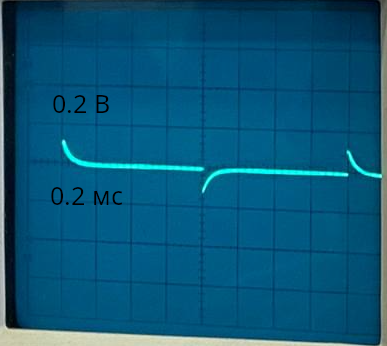
\includegraphics[width=0.8\linewidth]{5pp}
    \caption{апериодический режим в цепи 3-го порядка}
\end{figure}
\begin{enumerate}
    \item Процесс описывается выражением $f_2(t) = A_1e^{-25641t} + 
    A_2e^{-26166+i44892} + A_3e^{-26166-i44892}$
    \item $p_1 = -26166; \, p_{2,3} = -26166 \pm i44892$, частоты соотвествуют осциллограмме.
\end{enumerate}
\section{Вывод}
В лабораторной работе были изучены связи между видом свободного
процесса в цепи и расположением собственных частот 
(корней характеристического уравнения) на комплексной плоскости. 
Для второго порядка следующие закономерности вида процесса в 
зависимости от собственных частот: вещественные – апериодический, 
комплексно-сопряженные – периодический, кратные – критический. 
Экспериментально определены значения собственных частот и добротностей 
RLC-контуров по осциллограммам. 
\end{document}